\def\pgfsysdriver{pgfsys-dvipdfmx.def}   %некоторая поправка бага в связке xelatex - beamer.
\documentclass{beamer}

\usepackage[cm-default]{fontspec} % or install lmodern and remove cm-default opt
\usepackage{xunicode} % some extra unicode support
\usepackage{xltxtra} % \XeLaTeX macro
\usepackage{indentfirst} % I believe it is better for Russian

\usetheme{Madrid}
%\usepackage[utf8]{inputenc}
%\usepackage{pscyr}
\usepackage{cmap}
%\usepackage[T2A]{fontenc}
\usepackage[english,russian]{babel}
\usepackage{amssymb,amsfonts,amsmath,mathtext}
\usepackage{cite,enumerate,float,indentfirst}



\setromanfont{Charis SIL}
\setsansfont{Times New Roman}
\setmonofont{Times New Roman}
\setmainfont{Times New Roman} % this allows to use sans-serif as default font

\tolerance=1000
\emergencystretch=0.74cm
\hyphenation{классицис-ти-чес-кой}
\hyphenation{кирил-ли-чес-ких}


\title{Расчет скорости перехода между уровнями Ландау в наклонном магнитном поле в двойной квантовой яме.}
\author{Куцевол Андрей Александрович.}
\date{2012}


\newcommand{\beq}{\begin{equation}\begin{gathered}}
\newcommand{\beqn}{\begin{equation}\begin{gathered} \nonumber }
\newcommand{\eeq}{\end{gathered}\end{equation}}


\newcommand{\bdft}{\begin{dft}}
\newcommand{\edft}{\end{dft}}

\newcommand{\bexe}{\begin{exe}}
\newcommand{\eexe}{\end{exe}}

\newcommand{\brem}{\begin{rem}}
\newcommand{\erem}{\end{rem}}

\newcommand{\btrm}{\begin{trm}}
\newcommand{\etrm}{\end{trm}}
\newcommand{\angstr}{\stackrel{\circ}{\mathrm{A}}}

\newcommand{\bprf}{\begin{prf}}
\newcommand{\eprf}{\end{prf}}


\newcommand{\pal}{\partial}
\newcommand{\my}{\mu}

\newcommand{\hx}{\hspace{1ex}}
\newcommand{\hxx}{\hspace{2ex}}
\newcommand{\hxxx}{\hspace{3ex}}


\newcommand{\bfr}{\mathbf{r}}
\newcommand{\bft}{\mathbf{t}}
\newcommand{\bfn}{\mathbf{n}}
\newcommand{\bfm}{\mathbf{m}}
\newcommand{\bfi}{\mathbf{i}}
\newcommand{\bfj}{\mathbf{j}}
\newcommand{\bfk}{\mathbf{k}}
\newcommand{\bfb}{\mathbf{b}}
\newcommand{\bfx}{\mathbf{x}}
\newcommand{\bfy}{\mathbf{y}}
\newcommand{\bfz}{\mathbf{z}}
\newcommand{\bfu}{\mathbf{u}}
\newcommand{\bfl}{\mathbf{l}}
\newcommand{\vomg}{\vec{\omega}}

\begin{document}

\maketitle

%%%%%%%%%%%%%%%%%%%%%%%%%%%%%%%%%%%%%%%%%
\begin{frame}
\frametitle{Введение.}
\begin{block}{}

\end{block}
\end{frame}
%%%%%%%%%%%%%%%%%%%%%%%%%%%%%%%%%%%%%%%%%


%%%%%%%%%%%%%%%%%%%%%%%%%%%%%%%%%%%%%%%%%
\begin{frame}
\frametitle{Вспомним классическую кинематику.}
%%%%%%%%%%%%%%%%%%%%%
\begin{columns}[t]
\begin{column}{0.40\linewidth}
\begin{block}{Угловая скорость}
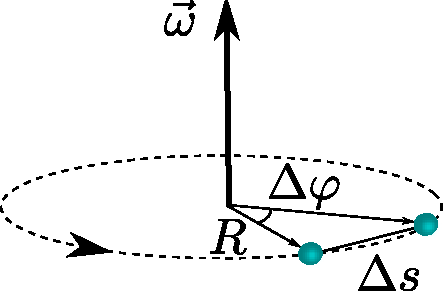
\includegraphics[width=1\columnwidth]{circ_motion}
\end{block}
\end{column}

\begin{column}{0.40\linewidth}
Если смотреть вслед вектору угловой скорости $\omega$ то вращение представляется происходящим по часовой стрелке.

\end{column}
\end{columns}
\begin{block}{Связь линейной и угловой скоростей.}
\beq \label{sav_v}
v = \lim _{\Delta t \rightarrow 0} \frac{\Delta s}{\Delta t} = \lim _{\Delta t \rightarrow 0}
\left(
R \frac{\Delta \varphi}{\Delta t}
\right) = R \lim _{\Delta t \rightarrow 0} \frac{\Delta \varphi}{\Delta t} = R \omega
\eeq
asdf
\end{block}
%%%%%%%%%%%%%%%%%%%%%
\end{frame}
%%%%%%%%%%%%%%%%%%%%%%%%%%%%%%%%%%%%%%%%%

\begin{frame}
\frametitle{Момент силы.}
%%%%%%%%%%%%%%%%%%%%%
\begin{columns}[t]
\begin{column}{0.40\linewidth}
\begin{block}{Угловая скорость}
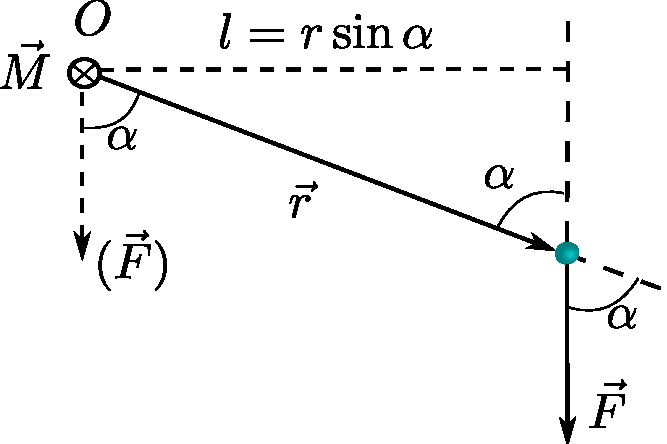
\includegraphics[width=1\columnwidth]{mom_sil}
\end{block}
\end{column}

\begin{column}{0.40\linewidth}
\begin{itemize}
\item
Модуль вектора $\vec{M}$
\beq
M = Fl = Fr \sin \alpha
\eeq
\item
Правовинтовая система:
\beq
\vec{M} = [\vec{r}, \vec{F}]
\eeq
\end{itemize}

\end{column}
\end{columns}
%%%%%%%%%%%%%%%%%%%%%
\end{frame}
%%%%%%%%%%%%%%%%%%%%%%%%%%%%%%%%%%%%%%%%%

%%%%%%%%%%%%%%%%%%%%%%%%%%%%%%%%%%%%%%%%%

\begin{frame}[r]
\frametitle{Момент импульса.}
%%%%%%%%%%%%%%%%%%%%%%
%\begin{columns}[t]
%\begin{column}{0.8\linewidth}
%\begin{block}{}
%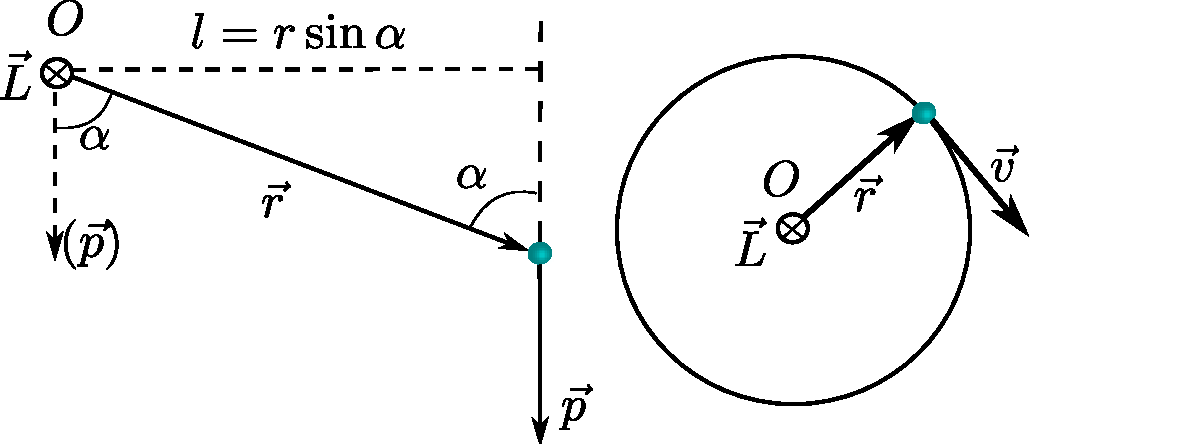
\includegraphics[width=1\columnwidth]{mom_imp}
%\end{block}
%\end{column}
%\end{columns}
%
%\begin{columns}[t]
%\begin{column}{0.45\linewidth}
%
%%\begin{block}{}
%\beqn
%\vec{L} = [\vec{r}, \vec{p}] = [\vec{r}, m \vec{v}]
%\eeq
%
%\beqn
%\frac{d}{dt} \vec{L} = \frac{d}{dt}[\vec{r}, m\vec{v}] = [\vec{r}, m \dot{\vec{v}} ] + [\dot{\vec{r}}, m \vec{v}]
%\eeq
%%\end{block}
%\end{column}
%
%\begin{column}{0.45\linewidth}
%%\begin{block}{}
%
%\beqn
%\frac{d}{dt} \vec{L} = [\vec{r}, \vec{F}] + [\vec{v}, m\vec{v}]
%\eeq 
%
%\beqn
%\frac{dL}{dt} = \vec{M}
%\eeq
%%\end{block}
%
%\end{column}
%\end{columns}
%
%%%%%%%%%%%%%%%%%%%%%%
\end{frame}
%%%%%%%%%%%%%%%%%%%%%%%%%%%%%%%%%%%%%%%%%

%%%%%%%%%%%%%%%%%%%%%%%%%%%%%%%%%%%%%%%%%

\begin{frame}[r]
\frametitle{Момент импульса.}
%%%%%%%%%%%%%%%%%%%%%
\begin{columns}[t]
\begin{column}{0.5\linewidth}
\begin{block}{}
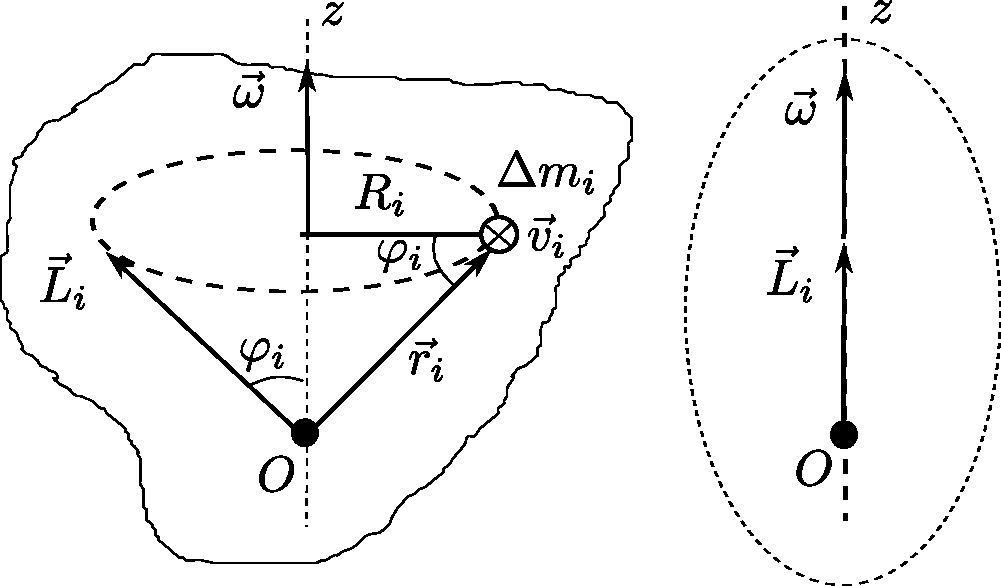
\includegraphics[width=1\columnwidth]{gyro}
\end{block}
\end{column}

\begin{column}{0.4\linewidth}
\beqn
L_{zi} = L_{i} \cos \varphi _{i}
\eeq
\beqn
L_{i} = \Delta m_{i}r_{i} \vec{v}_{i}
\eeq
\beqn
L_{zi} = \Delta m_{i} r_{i} v_{i} \cos \varphi_{i} = \\
= \Delta m_{i} R_{i} v_{i}
\eeq
\beqn
v_{i} = \omega R_{i};
\eeq
\beqn
L_{zi} = \omega R^{2}_{i} \delta m_{i} 
\eeq
\end{column}
\end{columns}

\bigskip

\beqn
L_{z} = \sum L_{zi} = \sum \omega R_{i}^{2} \Delta m_{i} = \omega \sum R_{i}^{2} \Delta m_{i}
\eeq

\beqn
I = \sum R_{i}^{2} \Delta m_{i}; \hxxx L_{z} = i\omega ;
\eeq

\beqn
\hxxx \vec{L} = I \omega - \text{для симметричного тела}.
\eeq

%%%%%%%%%%%%%%%%%%%%%
\end{frame}
%%%%%%%%%%%%%%%%%%%%%%%%%%%%%%%%%%%%%%%%%

\begin{frame}[r]
\frametitle{Гироскопы.}
\begin{columns}[t]
\begin{column}{0.5\linewidth}
\begin{block}{}
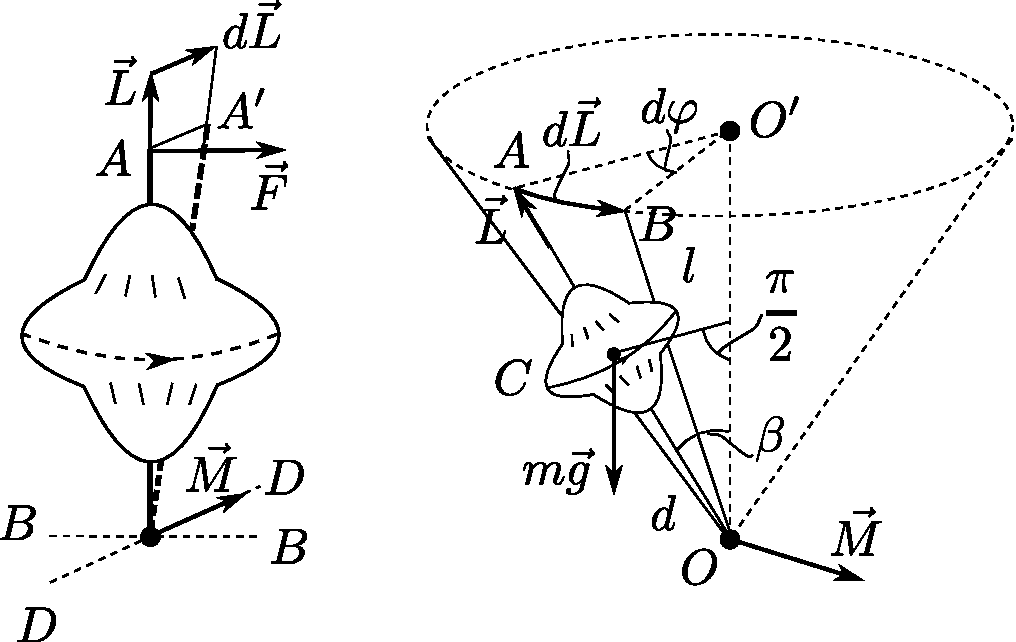
\includegraphics[width=1\columnwidth]{gyro2}
\end{block}
\end{column}
\begin{column}{0.45\linewidth}
\small{ В результате действия силы $\vec{F}$ в течении времени $dt$ момент импульса $\vec{L}$ получит приращение $d\vec{L} = \vec{M} dt$, где $\vec{M}$ - момент силы $\vec{F}$ относительно точки $O$. Новое значение момента импульса, равное $L + d\vec{L}$ окажется повернутым вокруг оси $BB$. Поскольку вектор $\vec{L}$ направлен вдоль оси гироскопа, вместе с $\vec{L}$ повернется и ось, перейдя из положения $OA$ в положение $OA'$. }
\end{column}
\end{columns}
\medskip
\small{Таким образом, в поле сил тяжести ось гироскопа с неподвижной точкой поворачивается вокруг вертикали, описывая конус. Такое движение гироскопа называется \textbf{прецессией}.}
\end{frame}

%%%%%%%%%%%%%%%%%%%%%%%%%%%%%%%%%%%%%%%%%

\begin{frame}[r]
\frametitle{Гиромагнитное соотношение.}
\begin{columns}[t]
\begin{column}{0.3\linewidth}
\begin{block}{}
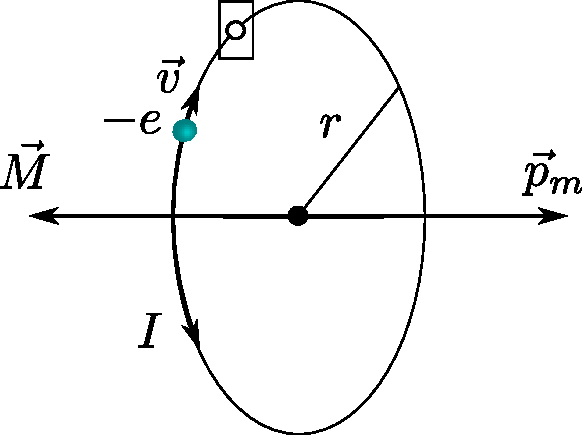
\includegraphics[width=1\columnwidth]{mag_mech}
\end{block}
\end{column}

\begin{column}{0.67\linewidth}
\scriptsize{Магнитный момент создаваемого электроном тока равен.
\beqn
p_{m} = IS = e\nu \pi r^{2} = \frac{evr}{2}
\eeq
и называется \textbf{орбитальным магнитным моментом}.

Вектор $p_{m}$ образует с направлением тока правовинтовую систему, а с направлением движения электрона левовинтовую.



Движущийся по орбите электрон обладает моментом импульса
\beqn
\vec{L} = [\vec{r}, m \vec{v}]
\eeq
}
\end{column}
\end{columns}
\scriptsize{
Вектор $\vec{L}$ называется орбитальным механическим моментомо элеткрона, и образует с направлением движения электрона правовинтовую систему.
Векторы $\vec{p}_{m}$ и $\vec{L}$ направлены противоположно. Отношение магнитного момента элементарной частицы к ее механическому называется гиромагнитным соотношением:
\beqn
\frac{p_{m}}{L} = - \frac{e}{2m}
\eeq
}
\end{frame}


%%%%%%%%%%%%%%%%%%%%%%%%%%%%%%%%%%%%%%%%%

\begin{frame}[r]
\frametitle{Почему собственный магнитный момент электрона?}
\begin{block}{}
\scriptsize{
Намагничивание магнетика приводит к его вращению - опыт Эйнштейна и де Хааса.

Вращение магнетика вызывает его намагничивание - опыт Барнетта.

Из данных опыта Эйнштейна и де Хааса было вычислено гиромагнитное соотношение которое оказалось равным
\beqn
\frac{p_{m}}{L} = - \frac{e}{m}
\eeq
Таким образом, знак заряда носителей, создающих молекулярные токи, совпадал со знаком заряда электрона. Однко полученный результат превысил ожидаемое значение в два раза. Из опыта Барнетт получил для гиромагнитного соотношения велечина, также в два раза превышающую теоретическое значение.  В дальнейшем выяснилось, что кроме орбительных моментов, электронон обладает собственным механическим и магнетным моментами, для которых гиромагнитное соотношениеравно
\beqn
\frac{p_{ms}}{M_{s}} = - \frac{e}{m}
\eeq
т.е. совпадает с экспериментальным значением.  Собственный магнитный момент электрона равен
\beqn
p_{m} = - \frac{e}{m}M_{s} = -\frac{e}{m}\frac{\hbar}{2} = - \frac{e \hbar}{2m}
\eeq
Величину
$\my _{B} = \frac{e \hbar}{2m}$
называют магнетоном Бора. Т.е. для электрона $M_{s} = \frac{1}{2}\hbar$
}
\end{block}
\end{frame}

\begin{frame}[r]
\frametitle{Ларморова прецессия.}
\begin{columns}[t]
\begin{column}{0.6\linewidth}
\begin{block}{}
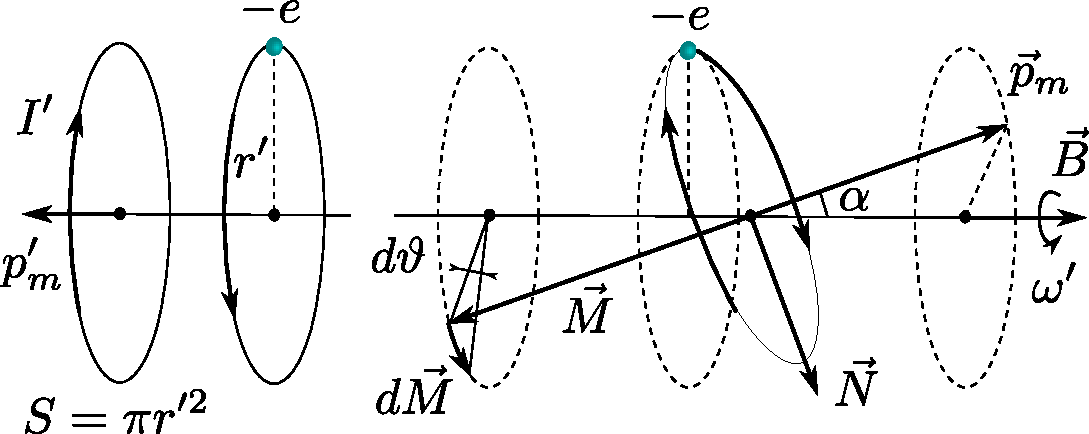
\includegraphics[width=1\columnwidth]{larmor}
\end{block}
\end{column}
\end{columns}

\medskip

\scriptsize{ $\vec{N} = [\vec{p}_{m}, \vec{B}]$ - Во внешнем магнитном поле $\vec{B}$ на орбиту действует вращательный момент, стремящийся установить орбитальный момент электрона $\vec{p}_{m}$ по направлению поля. Под действием момента $\vec{N}$ векторы $p_{m}$ и $\vec{M}$ совершают прецессию вокруг направления вектора магнитной индукции $\vec{B}$.
}

\end{frame}

\begin{frame}[r]
\frametitle{Скорость пецесии.}
\begin{block}{}
\scriptsize{
За время $dt$ вектор $\vec{M}$ получает приращение $d\vec{M}$ равное
\beqn
d \vec{M} = \vec{N}dt
\eeq
Вектор $d\vec{M}$ как и вектор $\vec{N}$, перпендикулярен к плоскости, проходящей через векторы $\vec{B}$ и $\vec{M}$; его модуль равен
\beqn
|d\vec{M}| = p_{m} B \sin \alpha dt
\eeq
где $\alpha$ - угол между $p_{m}$ и $\vec{B}$. За время $dt$ плоскость, в которой лежит вектор $\vec{M}$, повернется вокруг направления $\vec{B}$ на угол
\beqn
d \vartheta = \frac{|d \vec{M}|}{M \sin \alpha} = 
\frac{p_{m} B \sin \alpha dt}{M \sin \alpha} = 
\frac{p_{m}}{M} B dt
\eeq

Разделив этот угол на время $dt$, и подставляя выражение для гиромагнитного соотношения найдем угловую скорость прецессии:
\beqn \label{sav_57.1}
\omega_{L} = \frac{e B}{2m}
\eeq
\tiny{
Частоту $\omega_{L}$ называют частотой ларморовой прецессии. Она не зависит от угла наклона орбиты, от радиуса орбиты или скорости электрона и одинакова для всех электронов входящих в состав атома.
}
}
\end{block}
\end{frame}

\begin{frame}[r]
\frametitle{Диамагнетики и парамагнетики.}
\begin{block}{}
\scriptsize {
Магнитным мометном всего атома является векторная сумма орбитальных и спиновых магнитных моментов. Диамагнетами называются только те вещества, у которых атомы не обладают магнитным моментом.

Итак, под действием внешнего магнитного поля возникает прецессия электронных орбит с одинаковой для всех электронов угловой скростью.  Обусловленное прецессией дополнительное движение электронов приводит к возникновению индуцированного магнитного момента атома $p'_{m.at} = \sum p'_{m}$, направленного против поля. Таким образом в диамагнетиках внешнее магнитное поле ослабляется. Очедивно, что диамагнетизмом обладает любое вещество. Однако, в тех случаях, когда атомы обладают сами по себе магнитным моментом, магнитное поле не только индуцирует момент $p'_{m.at}$, но и оказывает на магнитные моменты атомов ориентирующее действие, устанавливая их по направлению пол. Результирующий момент оказывается положителен и вещество ведет себя как парамагнетик. Атом обладает в магнитном поле потенциальной энергией
\beqn
W = - p_{m} B \cos \vartheta
\eeq
Вероятность того, что магнитный момент атома будет образовывать с направлением вектора $\vec{B}$ угол, заключенный в ределах $\vartheta$ до $\vartheta + d \vartheta$, пропорциональна
\beqn
\exp {-\frac{W}{kT}} = \exp {\frac{p_{m} B \cos \vartheta}{kT}} - \text{Закон Больцмана}
\eeq
}
\end{block}
\end{frame}

\begin{frame}[r]
\frametitle{Явление ЭПР.}
\begin{columns}[t]
\begin{column}{0.45\linewidth}
\begin{block}{}
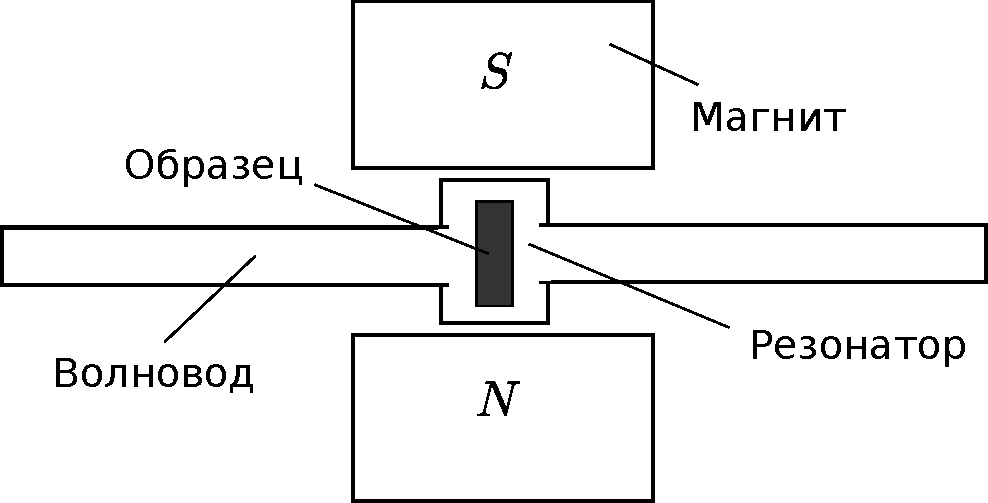
\includegraphics[width=1\columnwidth]{equip}
\end{block}
\end{column}

\begin{column}{0.45\linewidth}
\begin{block}{}
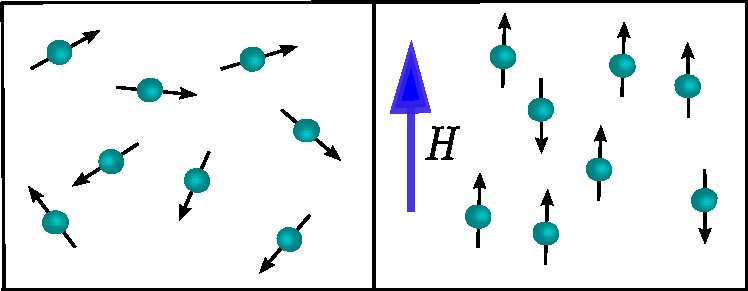
\includegraphics[width=1\columnwidth]{order}
\end{block}
\end{column}
\end{columns}

\medskip

\scriptsize{
В отсутствие поля все направления магнитных моментов равновероятны.

В магнитном поле минимум энергии достигается при совпадении $p_{m}$ с направлением вектора индукции, благодаря чему возникает преимущественная ориентация. Однако при действии самого поля переориентации не возникает: магнитный момент испытывает лишь прецессионное движение вокруг направления вектора магнитной индукции. Переориентировка магнитных моментов происходит в результате столконовений и взаимодействий атомов между собой.
}
\end{frame}

\begin{frame}[r]
\frametitle{Явление ЭПР. Эффект Зеемана}
\begin{columns}[t]
\begin{column}{0.3\linewidth}
\begin{block}{}
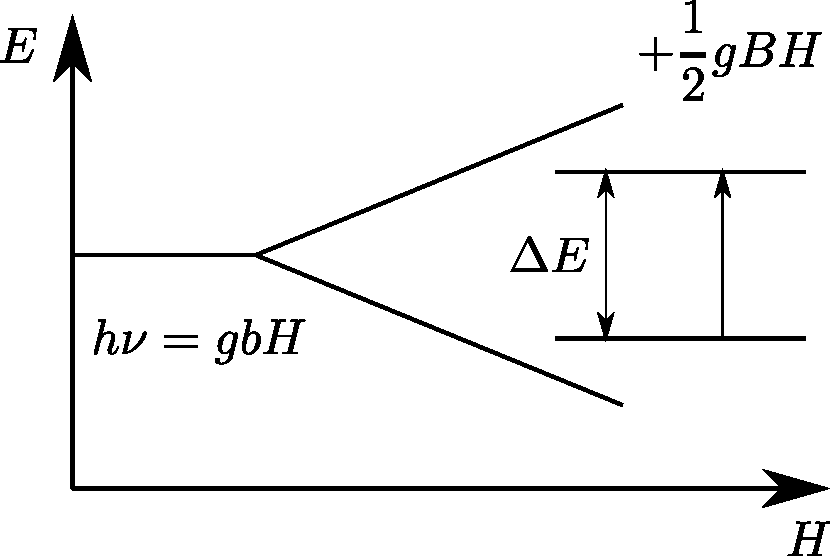
\includegraphics[width=1\columnwidth]{zeeman}
\end{block}
\end{column}

\begin{column}{0.65\linewidth}
\begin{block}{}
\scriptsize{
С приложением внешнего магнитного поля, магнитные моменты упорядочиваются относительно поля, и их энергетические уровни расщепляются. Для электронов с магнитными моментами ориентированными по полю $E_{s} = -\frac{1}{2}g \beta H$, против поля $E_{s} = +\frac{1}{2}g \beta H$.

Заселенность энергетических уровней определяется распределением Больцмана.
\beq \label{bolz1}
\frac{n_{\frac{1}{2}}}{n_{\frac{-1}{2}}} = \exp \frac{- \Delta E}{kT}.
\eeq
}
\end{block}
\end{column}
\end{columns}
\end{frame}

\begin{frame}[r]
\frametitle{Явление ЭПР. Резонанс.}
\begin{columns}[t]
\begin{column}{1\linewidth}
\begin{block}{}
\scriptsize {
Пусть в парамагнетике, помещенном в магнитное поле, создается дополнительное периодическое поле, вектор индукции которого перпендикулярен вектору индукции постоянного поля. За счет постоянного магнитного поля, моменты атомов совершают ларморову прецессию. В результате взаимодействия магнитного момента $\vec{p}_{m.at}$ с индукцией $\vec{B}$ дополнительного переменного магнитного поля создается момент сил $\vec{M}$ стремящийся изменить угол между $\vec{p}_{m.at}$ и $\vec{B}$. Если эта частота переменного магнитного поля отличатся от частоты ларморовой прецессии, то часть времени этот момент стремится увеличить угол а часть времени уменьшить, и в среднем никакого эфекта не наблюдается.

Если же частоты переменного магнитного поля и ларморовой прецессии совпадают, то в результате сравнительно длительного действия момента сил происходит переориентация магнитного момента атома и изменение угла между ним и вектором индукции постоянного магнитного поля. Это явление называется \textbf{парамагнитным резонансом}. Это явление называется парамагнитным резонансом. Переориентация сопровождается обменом энергией с переменным магнитным полем, вектор индукции которого перпендикулярен вектору индукции постоянного магнитного поля. При переориентировке с высших уровней будет \textbf{индуцированная эмиссия}, с нижних\textbf{ резонансное поглощение}.

\textbf{Вероятности переходов равны, но поглощение будет преобладать в силу распределения Больцмана.} Условием наступления парамагнитного резонанса является
\beqn
\Delta E = h\nu  = g \beta H
\eeq
}
\end{block}
\end{column}
\end{columns}
\end{frame}

%%%%%%%%%%%%%%%%%%%%%%%%%%%%%%
%%%%%%%%%%%%%%%%%%%%%%%%%%%%%%

\begin{frame}[r]
\frametitle{Характеристики спектров ЭПР.}
\begin{columns}[t]

\begin{column}{0.4\linewidth}
\begin{block}{}
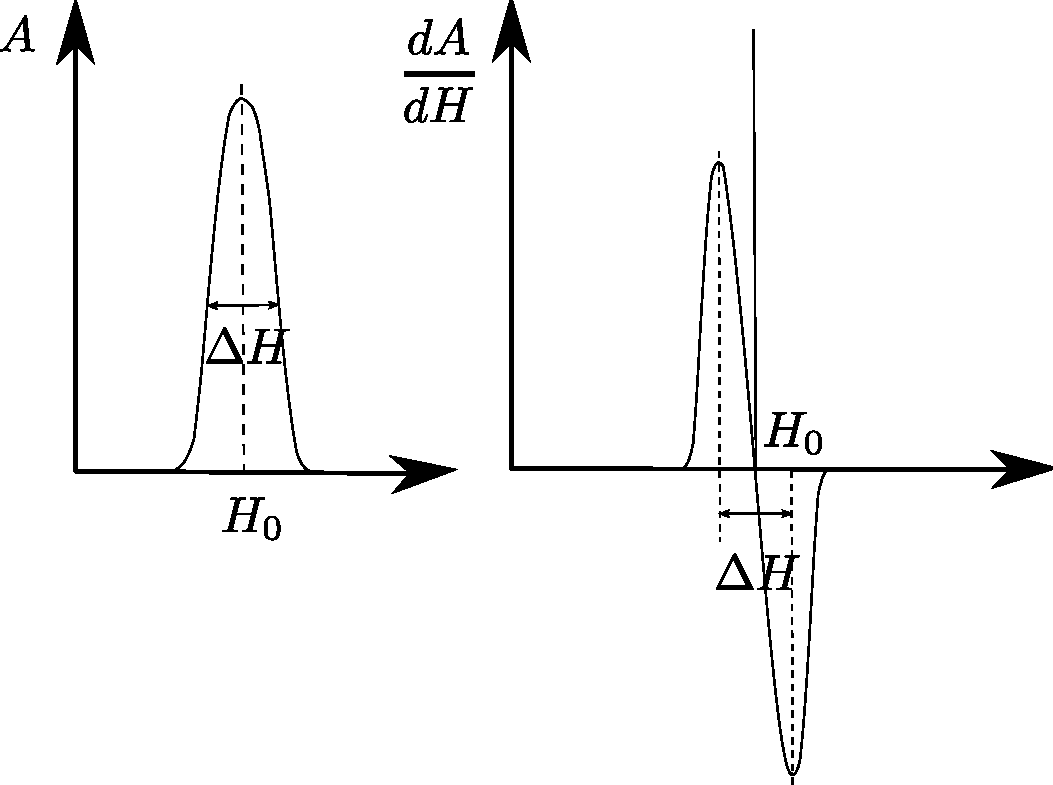
\includegraphics[width=1\columnwidth]{spectr}
\end{block}
\end{column}

\begin{column}{0.55\linewidth}
\scriptsize{
Сигнал ЭПР чаще всего представляется первой производной линии поглощения , в целях повышения точности определения максимумов поглощения.

%\textbf{Площадь под кривой} поглощения пропорциональна концентрации парамагнитных частиц в образце.
\beqn \label{conc}
C_{\text{изм}} = C_{\text{эт}} \frac{S_{\text{изм}}}{S_{\text{эт}}}
\eeq
\medskip
\textbf{Форма линии.} Хотя, в соответствии с основным условием резонанса (\ref{res1}), поглощение происходит при равенстве кванта энергии и разнице энергий между уровнями неспаренных электронов, спектр ЭПР не линейчатый а непрерывный в окрестности точки резонанса.

}
\end{column}
\end{columns}



\scriptsize{

\textbf{Ширина линии спектра ЭПР}. Ширина спектра ЭПР зависит от взаимодействия магнитного момента электрона с магнитными моментами окружающих ядер (решетки) и электронов. Рассмотрим механизм поглощения энергии неспаренными электронами подробнее. Если в низкоэнергетическом состоянии находится $N_{1}$ электронов, а в высокоэнергетическом $N_{2}$ и $N_{1} > N_{2}$, то и при подаче электромагнитной энергии на образец разность заселенности уровней будет уменьшатся пока не станет равной нулю.
}

\end{frame}

%%%%%%%%%%%%%%%%%%%%%%%%%%%%%%%%%%%%%%%%%%%%%

\begin{frame}[r]
\scriptsize{
Это происходит потому, что вероятности одиночного перехода под действием излучения из низкоэнергетического состояния в высокоэнергетическое и наоборот ($W_{12}$  и $W_{21}$ равны между сообой, а заселенность нижнего уровня выше. Введем перменную $n = N_{1} - N_{2}$. Тогда изменение разности заселенности уровней во времени можно записать
\beqn
\frac{d N_{1}}{dt} = N_{2}W_{21} - N_{1}W_{12} \hx \text{и} \hx \frac{d N_{2}}{dt} = N_{1}W_{12} - N_{2}W_{21}; \hx \text{откуда}
\eeq

\beqn \label{utro_5.24}
\frac{dn}{dt} = \frac{d N_{1}}{dt} - \frac{dN_{2}}{dt} = -2W (N_{1} - N_{2}) = -2Wn
\eeq
Однако, в эксперименте \textbf{изменения разности} заселенности уровней не наблюдается благодаря тому, что существуют процессы релаксации, поддерживающие постоянной эту разность. Механизм релаксации заключается в передаче кванта электромагнитной энергии решетке или окружающим электронам и возвращения электона на низкоэнергетический уровень. Если обозначить вероятности переходов индуцируемых решеткой через $P_{12}$ и $P_{21}$, причем $P_{12} < P_{21}$, то изменение разности заселенности уровней будет
\beqn \label{utro_5.25}
\frac{dn}{dt} = -2 (N_{1}P_{12} - N_{2}P_{21})
\eeq
или если заменить $N_{1} + N_{2}$ на $N$, то
\beqn \label{utro_5.26}
\frac{dn}{dt} = N(P_{21} - P_{12}) - n(P_{12} + P_{21}).
\eeq
}
\end{frame}

\begin{frame}[r]
\scriptsize{
В стационарном состоянии, когда изменение разности заселенности равно нулю, начальная разность заселенностей уровней ($n_{0}$) остается постоянной и равной
\beq \label{utro_5.27}
n_{0} = N \frac{P_{21} - P_{12}}{P_{12} + P_{21}}
\eeq

В этом случае 
\beq \label{utro_5.28}
\frac{dn}{dt} = (n_{0} -n)(P_{12} + P_{21}),
\eeq
или заменив $(P_{12} + P_{21}$ на $\frac{1}{T_{1}}$, получим
\beq \label{utro_5.29}
\frac{dn}{dt} = \frac{n_{0} - n}{T_{1}}
\eeq

\textbf{Величина $T_{1}$ называется временем спин-решеточной релаксации} и характеризует среднее время жизни спинового состояния. В итоге, изменение разности заселенности уровней системы наспаренных электронов, находящейся под воздействием электромагнитного излучения и взаимодействующей с решеткой, будет определятся уровнением
\beq \label{utro_5.30}
\frac{dn}{dt} = -2Wn + \frac{n_{0} - n}{T_{1}}
\eeq

Отсюда следует, что в стационарном состоянии
\beq \label{utro_5.31}
n = \frac{n_{0}}{1+ 2WT_{1}}
\eeq
и при $2WT_{1} << 1$, $n = n_{0}$	, т.е. при относительно небольших мощностях разность заселенности уровней остается практически постоянной.
}
\end{frame}

\begin{frame}
\scriptsize{
Из соотношения неопределенностей Гейзенберга следует, что
\beq \label{utro_5.32}
\Delta E \geqslant \frac{h}{2\pi} \times \frac{1}{T_{1}},
\eeq

Если принять, что $\Delta t$ равно $T_{1}$, а $\Delta E$ соответствует $g\beta \Delta H$, то уравнение (\ref{utro_5.32}) можно переписать в вдие
\beq \label{utro_5.33}
\Delta H \geqslant \frac{h}{2\pi g \beta} \times \frac{1}{T_{1}}
\eeq
\textbf{т.е. неопределенность в ширине линии обратно пропорциональна времени спин-решеточной релаксации.}

Кроме взаимодействия магнитного момента неспаренного электрона с решеткой возможно, также его взаимодействие с магнитными моментами других электронов. Это взаимодействие приводит к уменьшению времени релаксации и тем самым к уширению линии спектра ЭПР. \textbf{В этом случае вводят понятие времени спин-спиновой релаксации ($T_{2}$).}

Наблюдаемое время релаксации считают суммой времени спин-решеточной и спин спиновой релаксации.
\beqn
\Delta H \geqslant \frac{h}{2\pi g \beta} \times \frac{1}{T_{eff}} = \frac{h}{2\pi g \beta} \times \frac{2T_{1} + T_{2}}{2T_{1}T_{2}}
\eeq

Для свободных радикалов в растворах $T_{1} >> T_{2}$, следовательно ширина линии будет определятся $T_{2}$. \textbf{Среди механизмов уширения линии} следует упомянуть следующие; диполь-дипольное взаимодействие; анизотропия $g$-фактора; динамичесоке уширение линии спиновый обмен.
}
\end{frame}

\begin{frame}
\scriptsize{
В основе \textbf{диполь-дипольного} взаимодействия лежит взаимодействие магнитного момента неспаренного электрона \textbf{с локальным магнитным полем}, создаваемым соседними электронами и ядрами. Напряженность магнитного поля в какой-либо точке зависит от расстояния до этой точки и взаимной ориентации магнитных моментов неспаренного электрона и другого взаимодействующего электрона или ядра. Изменение энергии неспаренного электрона будет определяться:
\beq \label{utro_5.34}
\Delta E = h \Delta \nu = g \beta \Delta H = g \beta \frac{\my}{R^{3}} (3 \cos ^{2} \theta - 1)
\eeq
где $\my$ - магнитный момент электрона, $R$ - расстояние, до источника локального магнитного поля, $\theta$ - угол между взаимодействующими магнитными моментами.

Локальное поле в любом данном узле будет зависеть от расположения соседей и от направлений их дипольных моментов. Локальное поле изменяется от узла к узлу, приводя к случайному смещению резонансной частоты каждого иона, которое аналогично смещению вследствие неоднородности внешнего магнитного поля. По этой причине рассмотренный эффект известен как \textbf{ `` неоднородное уширение линии '}'; резонансная частота каждого иона смещается, но время жизни данного квантового состояния иона не уменьшается.

Если парамагнитные ионы тождественны и их моменты прецессируют с одной и той же частотой во внешнем магнитном поле, то между ними существует добавочное  резонансное взаимодействие. прецессирующие компоненты одного магнитного момента создают осциллирующее поле в месте нахождения другого, которое имеет как раз необходимую частоту, чтобы вызвать магнитные резонансные переходы, и наоборот.
}
\end{frame}

\begin{frame}
\scriptsize{ При этом взаимодействие инудцирует резонансные переходы, которые эквивалентны обмену квантами между соседними ионами (в сильном внешнем поле этот обмен сохраняет энергию системы постоянной). Это добавочное взаимодействие тождественных спинов приводит к дополнительному уширению линии (которое по величине может составлять около $50 \%  $); оно также укорачивает время жизни отдельного иона в определенном квантовом состоянии, и уширение уже больше \textbf{ не является полностью} `` неоднородным ''. В случае чисто неоднородного уширения величина ($T_{2}$) не определена и не связана простым соотношением с наблюдаемой шириной линии.

\textbf{Вклад анизотропии g-фактора} в уширение линии ЭПР связан с тем, что орбитальное движение электрона создает переменнное магнитное поле с которым взаимодействует спиновый магнитный момент. Это взаимодействие приводит к отклонению g-фактора от значения  $ 2,0023$, соответствующего свободному электрону. Для кристаллических образцов величины g-фактора, соответствующие ориентации кристалла обозначают $g_{xx}, g_{yy}$ и $g_{zz}$ соответственно. При быстром движении молекул, например в растворах, анизотропия g-фактора может усредняться.

Спиновый обмен является еще одним способом уширения сигнала ЭПР. Механизм уширения сигнала при спиновом обмене заключается в изменении направления спинового магнитного момента электрона на противоположное при соударении с другим неспаренным электроном или иным парамагнетиком. Поскольку при таком соударении уменьшается время жизни электрона в данном состоянии, то сигнал ЭПР уширяется. Наиболее частным случаем уширения линии ЭПР по механизму спинового обмена является уширение сигнала в присутствие кислорода или парамагнитных ионов металлов.
}
\end{frame}

\begin{frame}
\frametitle{Литература.}
\begin{block}{}
1. A. Abragam, B.Bleaney. Electron paramagnetic resonance of transition ions. Oxford 1970.

2. И.В. Савельев. Курс физики. Т1.

3. И.В. Савельев. Курс физики. Т2.

4. А.Н. Матвеев. Электричество и магнетизм.

5. А.Н. Осипов. Метод электронного парамагнитного резонанса.
\end{block}
\end{frame}



%%%%%%%%%%%%%%%%%%%%%%%%%%%%%%%%%%%%%%%%%%%%%
%%%%%%%%%%%%%%%%%%%%%%%%%%%%%%%%%%%%%%%%%%%%%
%%%%%%%%%%%%%%%%%%%%%%%%%%%%%%%%%%%%%%%%%%%%%
%%%%%%%%%%%%%%%%%%%%%%%%%%%%%%%%%%%%%%%%%%%%%

%\begin{frame}[r]
%\frametitle{Ларморова прецессия.}
%\begin{columns}[t]
%\begin{column}{0.6\linewidth}
%\begin{block}{}
%%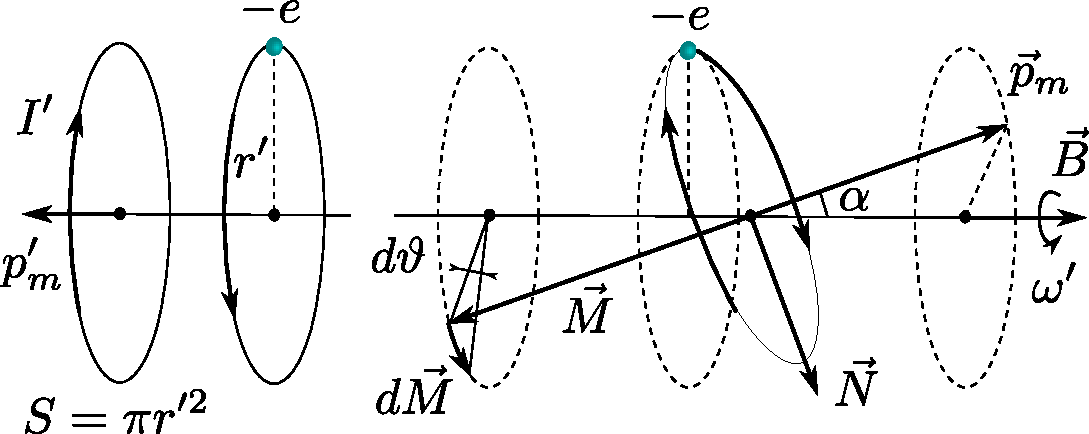
\includegraphics[width=1\columnwidth]{larmor}
%\end{block}
%\end{column}
%\end{columns}
%\end{frame}

\end{document}
